\def \eng #1{\foreignlanguage{english}{#1}}

\noindent\textbf{Цель работы.}
\begin{enumerate}
\item Ознакомление с возможностями ПЛИС и среды разработки цифровых устройств для ПЛИС.
\item Практическое ознакомление с разработкой простых управляющих устройств для ПЛИС \eng{Xilinx}.
\end{enumerate}

\section{Теоретические сведения}

\subsection{Цифровые устройства и их описание}

Комбинационным устройством называется такое устройство, значения выходных сигналов которого в данный момент времени определяются только значениями его входных сигналов в тот же момент времени. Иными словами, комбинационное устройство представляет собой устройство, не содержащее в себе элементов памяти.

Устройства, значения выходных сигналов которых зависят не только от значений входных сигналов в данный момент времени, но и от некоторой предыстории входных сигналов, называют последовательностными устройствами, или устройствами с памятью.

%Для комбинационных устройств существует простой и наиболее полный способ описания их работы, называемый таблицей истинности. Для последовательностных устройств наиболее адекватным является описание в виде таблицы состояний путем перечисления возможных переходов между состояниями с указанием значений входных сигналов и состояния устройства, при котором происходит данный переход, а также соответствующие новому состоянию значения выходных сигналов. В отличие от таблиц истинности (состояний) временные диаграммы показывают работу устройств во временной области.

Входные сигналы, воспринимаемые лишь в моменты перепадов тактового сигнала, называются тактируемыми, или синхронными. Это означает, что любые изменения внутреннего состояния последовательностного устройства, к которым они могут привести, происходят только в моменты перепадов тактового сигнала (в реальных устройствах --- устанавливаются к моменту перепада тактового сигнала).

Существуют устройства и с асинхронными входами. Асинхронные входные сигналы непрерывным образом влияют на состояние устройства, и наличие в сигнале промежутков времени, в течение которых происходит установление сигнала, может привести к неожиданным последствиям.

\subsection{Базовая библиотека \eng{Xilinx}}

Для схемотехнического проектирования применяется программный пакет \eng{Xilinx ISE}. Рассмотрим некоторые элементы библиотеки компонентов \eng{Xilinx ISE} (\autoref{fig:xilinxlib}).

\begin{figure}[h]%
\centering
%
\subfloat[][]{%
\label{fig:xilinxlib-comp}%
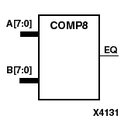
\includegraphics[width=0.15\textwidth]{comp}}%
\hspace{8pt}%
%
\subfloat[][]{%
\label{fig:xilinxlib-dflipflop}%
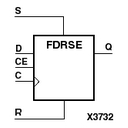
\includegraphics[width=0.15\textwidth]{dflipflop}}%
\hspace{8pt}%
%
\subfloat[][]{%
\label{fig:xilinxlib-counter}%
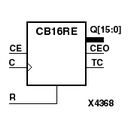
\includegraphics[width=0.15\textwidth]{counter}}%
\hspace{8pt}%
%
\subfloat[][]{%
\label{fig:xilinxlib-decoder}%
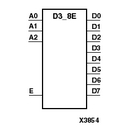
\includegraphics[width=0.15\textwidth]{decoder}}%
\hspace{8pt}%
%
\subfloat[][]{%
\label{fig:xilinxlib-mux}%
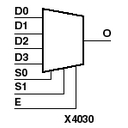
\includegraphics[width=0.15\textwidth]{mux}}%
\hspace{8pt}%
%
\subfloat[][]{%
\label{fig:xilinxlib-rom}%
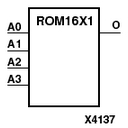
\includegraphics[width=0.15\textwidth]{rom}}%
\hspace{8pt}%
%
\caption[Компоненты базовой библиотеки.]{Примеры компонентов базовой библиотеки:
\subref{fig:xilinxlib-comp} Компаратор; %
\subref{fig:xilinxlib-dflipflop} \eng{D}-триггер; %
\subref{fig:xilinxlib-counter} Счетчик; %
\subref{fig:xilinxlib-decoder} Дешифратор; %
\subref{fig:xilinxlib-mux} Мультиплексор; %
\subref{fig:xilinxlib-rom} Постоянная память}%
\label{fig:xilinxlib}%
\end{figure}

\subsubsection{Компараторы}

Представляют собой комбинационные устройства, предназначенные для сравнения чисел. Выходной сигнал \eng{EQ} принимает значение \enquote{1}, если значения на входах \eng{A} и \eng{B} совпадают, и значение \enquote{0} в противном случае.

\subsubsection{Триггеры и регистры}

В базовой библиотеке представлено большое количество триггеров и регистров различного типа и разрядности. Регистры представляют собой несколько параллельно подключенных \eng{D}-триггеров.

\eng{D}-триггеры представляют собой последовательностное устройство, являющееся элементарной ячейкой памяти емкостью 1 бит. \eng{T}-триггер --- последовательностное устройство, являющееся элементарным 1-битным счетчиком.

\eng{JK}-триггер является \enquote{обобщением} \eng{D}- и \eng{T}-триггеров.

\subsubsection{Счетчики}

Счетчики представляют собой последовательностные устройства, предназначенные для генерации нарастающего или убывающего счетного кода. Тактовый сигнал \eng{C} определяет моменты времени, в которые возможно изменение состояния счетчика. Наращивание состояния счетчика возможно только при наличии \enquote{1} на входе разрешения счета \eng{CE}. Если значение счетного кода достигает максимально возможного, сигнал \eng{TC} принимает значение \enquote{1}. Сигнал \eng{CEO} определяет моменты времени, в которые должен нараститься следующий за этим каскад счетчиков. Если значение кода достигло максимально возможного, и сигнал разрешения счета \eng{CE} установлен в \enquote{1}, то по правилам счета значение счетчика должно перейти в начальное, а следующий каскад счетчиков должен нарастить свое значение на \enquote{1}.

\subsubsection{Логические элементы}

В библиотеке компонентов среды разработки присутствует большое количество различных логических элементов, среди которых вентили \enquote{И}, \enquote{ИЛИ}, \enquote{И-НЕ}, \enquote{ИЛИ-НЕ}, \enquote{НЕ}, \enquote{Исключающее ИЛИ}, \enquote{Исключающее ИЛИ-НЕ}, \enquote{И-ИЛИ}.

\subsubsection{Дешифраторы}

Дешифраторы представляют собой комбинационные элементы для декодирования входного числового кода в позиционный.

\subsubsection{Мультиплексоры}

Мультиплексоры представляют собой комбинационные элементы для мультиплексирования сигналов (подключения к выходному сигналу одного из нескольких входных сигналов). Управляющие сигналы \eng{S} определяют, какой из входных сигналов \eng{D} подключить к выходному сигналу \eng{O}. Управляющий сигнал \eng{E} разрешает или запрещает выдачу на выход значения одного из входных сигналов.

\subsubsection{Память}

В базовой библиотеке память представлена различными элементами \eng{ROM --- Read-Only Memory} и \eng{RAM --- Random Access Memory}. Сигналы \eng{A} и \eng{DPRA} обозначают адрес записываемого или считываемого слова. Сигналы \eng{WE} и \eng{D} обозначают соответственно разрешение записи и записываемые данные. Сигналы \eng{O}, \eng{SPO} и \eng{DPO} --- считываемые данные.

\subsection{Динамическая индикация}

Для уменьшение числа сигнальных линий, используемых для управления устройствами отображения, применяется так называемая динамическая, или непрерывная, индикация. Уменьшение числа линий достигается путем использования процедуры сканирования (последовательного перебора всех элементов) системы индикации с одновременным заданием состояния для выбранного в процедуре сканирования в данный момент элемента. Сканирование подразумевает наличие блока, перебирающего все возможные элементы системы индикации с определенной частотой, т.е. формирующего коды, соответствующие элементам системы индикации. Таким образом, динамическая индикация требует передачи индикатору кода, определяющего номер выделенного элемента (адрес элемента), а также сигнала состояния выделенного элемента.

\subsection{Лабораторная установка}

Для выполнения лабораторных работ используется лабораторная установка (\autoref{fig:model}), оснащенная интерфейсами для связи с ПК и разъемами расширения, а также приставка \enquote{блок динамической индикации}.

\begin{figure}[h]%
\centering
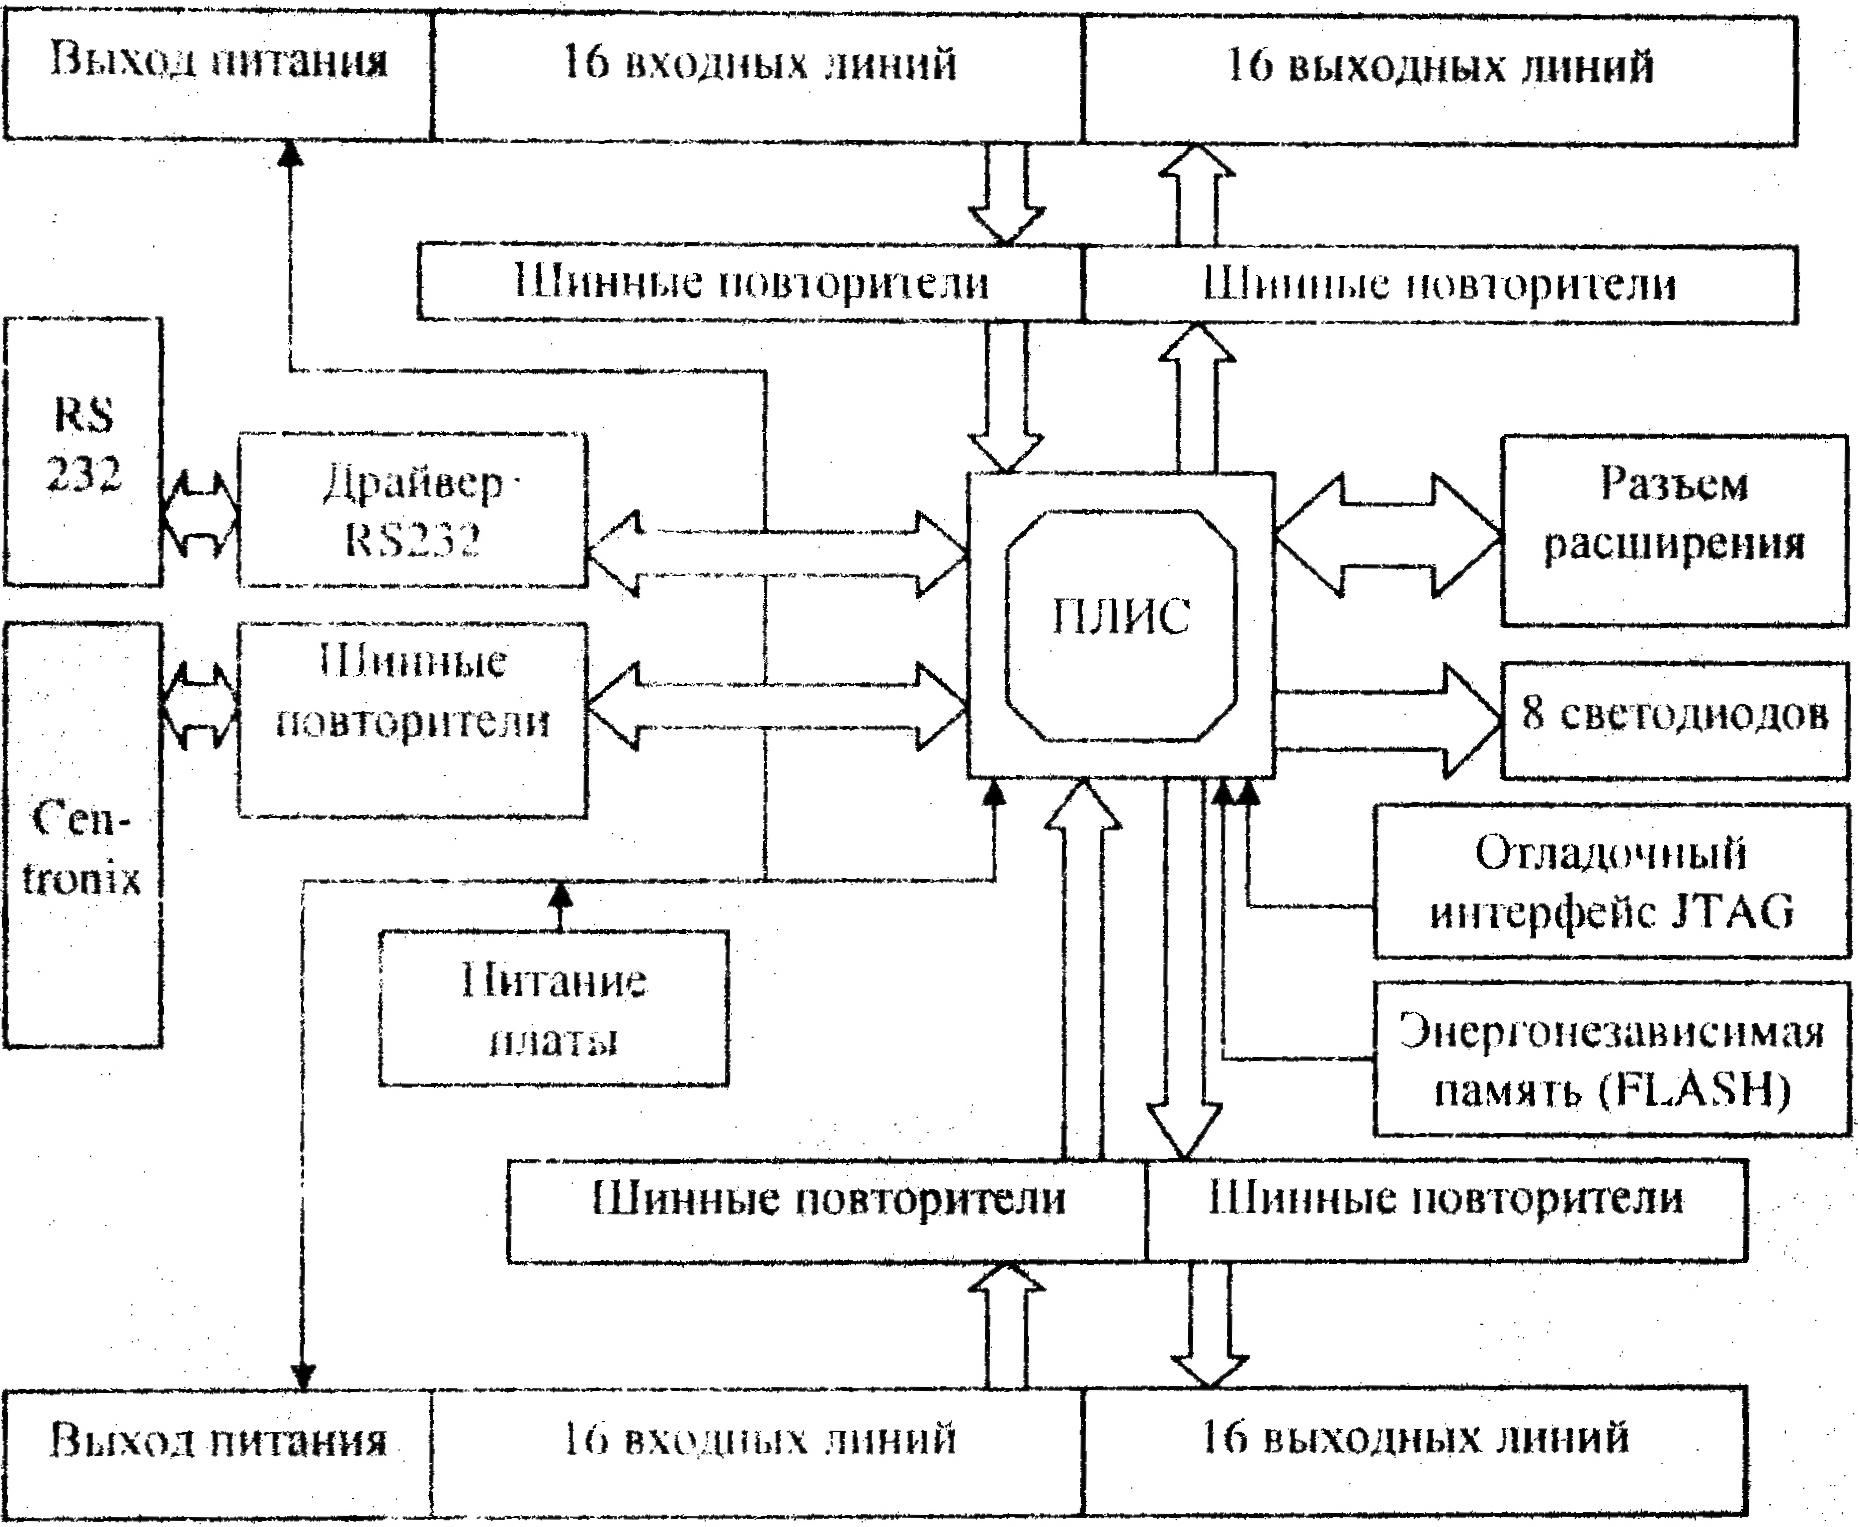
\includegraphics[width=0.6\textwidth]{model}%
\caption[Лабораторная установка.]{Лабораторная установка}%
\label{fig:model}%
\end{figure}

Приставка оснащена четырьмя семисегментными индикаторами, входом внешнего сигнала и звуковым динамиком.

\section{Методика эксперимента\label{sec:task}}

Предлагается при помощи описанного аппаратного лабораторного комплекса разработать следующие схемы цифровых устройств.

\begin{enumerate}[labelindent=\parindent,leftmargin=*]

\item Индикация цифровых эффектов на светодиодах.

\begin{enumerate}[label=\asbuk*)]

\item Эффект \enquote{бегущая тень}. Включен всегда только один из светодиодов. Номер включенного светодиода наращивается каждую секунду на единицу от 0 до 7. Когда номер светодиода переходит через значение 7, эффект начинается с начала.

\item Эффект \enquote{бегущая тень - 2}. Когда номер светодиода переходит через значение 7, эффект повторяется в обратном направлении --- каждую секунду номер включенного светодиода уменьшается на единицу до значения 0, после которого все повторяется с начала.

\item \enquote{Счетный код Джонсона}. Включаются по очереди все светодиоды от 0 до 7 с интервалом времени в 1 с. Через 1 с после включения светодиода №7 светодиоды с 0 по 7 по очереди должны выключиться также с интервалом в 1 с. После выключения седьмого светодиода эффект начинается с начала.

\item \enquote{Произвольный эффект}. Состояние светодиодов в каждый момент времени задается при помощи блока памяти.

\end{enumerate}

\item Частотомер.

Реализация устройства измерения частоты периодического сигнала и индикация полученного значения частоты на индикаторах приставки \enquote{блок динамической индикации}. Если на вход подается сигнал частоты, превышающей разрешение частотомера, требуется отобразить на блоке индикаторов сообщение об ошибке и подать звуковой сигнал.

\end{enumerate}

После синтеза схемы производится генерация файла прошивки и загрузка его в ПЛИС.

\section{Результаты и их обсуждение}

В ходе работы были реализованы два проекта в среде разработки \eng{Xilinx ISE}, отвечающие приведенным в \autoref{sec:task} заданиям. Рассмотрим их по порядку.

\subsection{Индикация цифровых эффектов}

\begin{figure}[h]%
\centering
%
\subfloat[][]{%
\label{fig:digeffects-mux}%
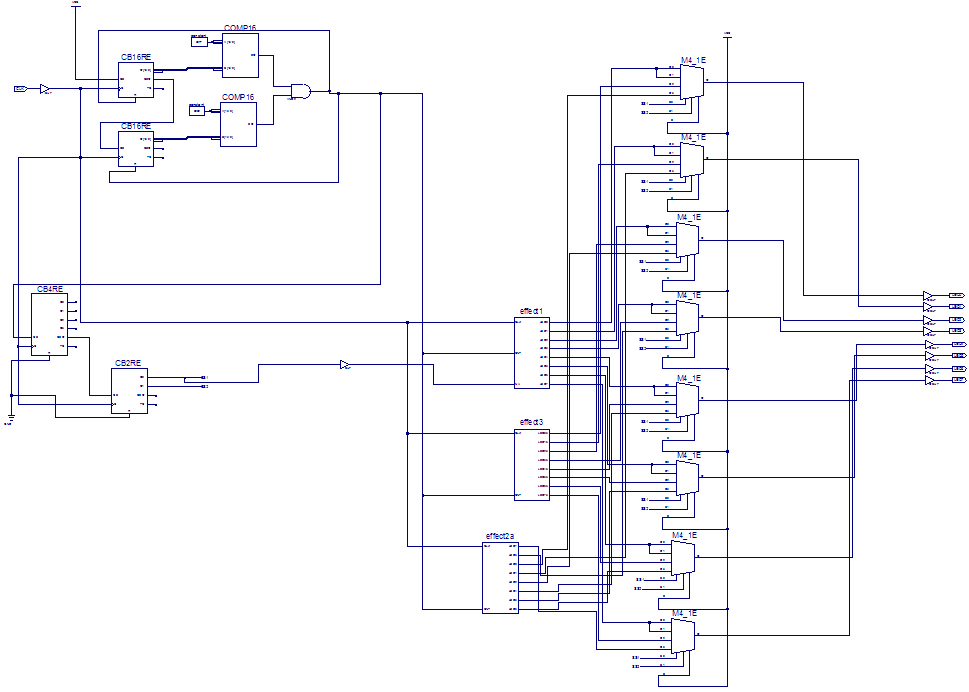
\includegraphics[width=0.8\textwidth]{leds-0}}%
\hspace{8pt}%
%
\subfloat[][]{%
\label{fig:digeffects-shade}%
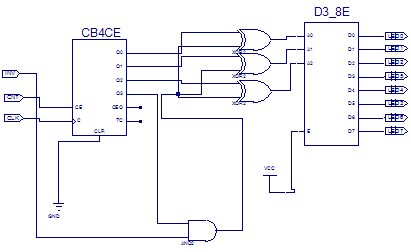
\includegraphics[width=0.3\textwidth]{leds-1}}%
\hspace{8pt}%
%
\subfloat[][]{%
\label{fig:digeffects-johnson}%
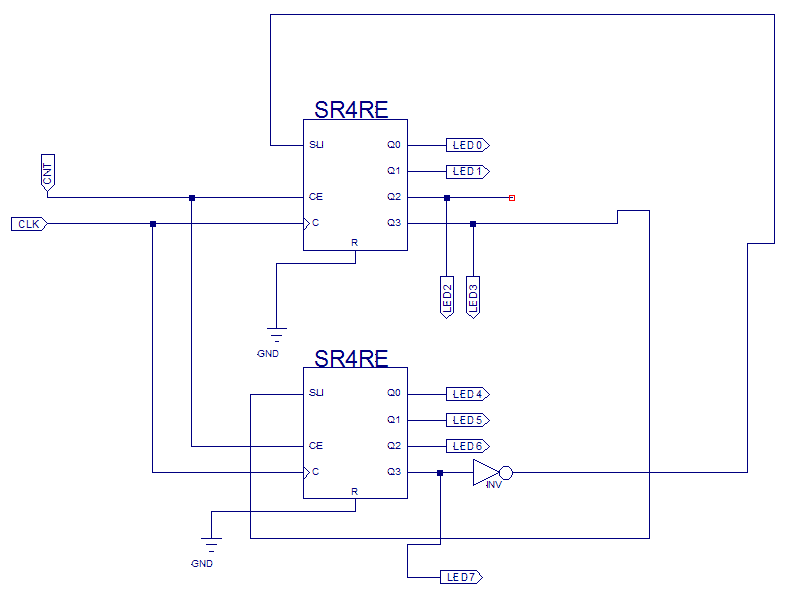
\includegraphics[width=0.3\textwidth]{leds-2}}%
\hspace{8pt}%
%
\subfloat[][]{%
\label{fig:digeffects-mem}%
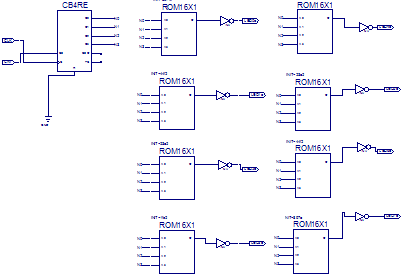
\includegraphics[width=0.3\textwidth]{leds-3}}%
\hspace{8pt}%
%
\caption[Схемы цифровых эффектов.]{Схемы цифровых эффектов:
\subref{fig:digeffects-mux} схема формирования временных интервалов и мультиплексирования эффектов; %
\subref{fig:digeffects-shade} схема эффекта \enquote{бегущая тень}; %
\subref{fig:digeffects-johnson} схема эффекта \enquote{счетный код Джонсона}; %
\subref{fig:digeffects-mem} схема \enquote{произвольного эффекта}} %
\label{fig:digeffects}%
\end{figure}

Был разработан проект для демонстрации четырех требуемых эффектов. Проект состоит из четырех схем (\autoref{fig:digeffects}):
%
\begin{enumerate*}[label=\asbuk*)]

\item схема формирования временных интервалов и мультиплексирования эффектов,

\item схема эффекта \enquote{бегущая тень} с возможностью смены направления \enquote{движения} эффекта,

\item схема эффекта \enquote{счетный код Джонсона},

\item схема \enquote{произвольного эффекта}.
\end{enumerate*}
%
Последние три преобразованы в схемные символы и импортированы в мультиплексор эффектов как обычные элементы библиотеки компонентов.

\subsubsection{Схема формирования временных интервалов и мультиплексирования эффектов\label{sec:time-interval-generator}}

Данная схема состоит из следующих частей.

\begin{enumerate}[label=\asbuk*)]

\item Схема формирования секундных временных интервалов формирует импульсы частотой один импульс в секунду (1Гц). Предназначена для определения моментов времени переключения состояния светодиодов. Выполнена на двух последовательно включенных 16-разрядных счетчиках и двух компараторах. На тактовый вход первого счетчика поступает тактовый сигнал, импульсы которого считаются и сравниваются компараторами с константой, на единицу меньшей количества тактовых импульсов в секунду, т.е. численно равной частоте тактового сигнала минус один. При равенстве значения счетного кода константе счетчики сбрасываются при следующем перепаде тактового сигнала.

\item Схема формирования 16-секундных временных интервалов формирует импульсы частотой один импульс в 16 секунд. Предназначена для определения моментов времени переключения эффектов. Выполнена на одном 4-разрядном счетчике в виде делителя частоты 1Гц, получаемой со схемы формирования секундных временных интервалов, на 16.

\item Схема мультиплексирования эффектов. Предназначена для выбора текущего демонстрируемого эффекта. Выполнена на одном 2-разрядном счетчике и восьми 4-мультиплексорах. Счетный код счетчика определяет номер эффекта. Счетчик наращивается каждые 16 секунд импульсами со схемы формирования 16-секундных временных интервалов. Счетный код используется для управления мультиплексорами, подключающими текущий эффект к выходу на светодиоды.

\end{enumerate}

\subsubsection{Эффект \enquote{бегущая тень}}

Данный эффект реализован на одном 4-разрядном счетчике и одном 3-разрядном дешифраторе. Младшие три разряда счетчика определяют номер $n$ активного светодиода. Старший разряд при наличии управляющего сигнала разрешения определяет направление \enquote{движения} эффекта, складываясь по модулю 2 с каждым разрядом номера $n$ светодиода, тем самым инвертируя его. Дешифратор в зависимости от поданного на его вход номера $m$ светодиода выдает на $m$-й выход логическую единицу, тем самым отключая $m$-й светодиод.

Наличие управляющего входа позволяет использовать данную схему и как реализацию эффекта \enquote{бегущая тень} (при отсутствии управляющего сигнала), и как реализацию эффекта \enquote{бегущая тень - 2} (при наличии управляющего сигнала).

\subsubsection{Эффект \enquote{счетный код Джонсона}}

Эффект реализован на двух последовательно соединенных 4-разрядных сдвиговых регистрах с линейной обратной связью (РСЛОС). Позиции нулей в коде, записанном в регистрах, определяют номера включенных светодиодов. Обратная связь берется со старшего разряда старшего регистра и подается через инвертор на последовательный вход данных младшего регистра.

\subsubsection{\enquote{Произвольный эффект}}

Для реализации эффекта используется 4-разрядный счетчик и восемь элементов постоянной памяти \eng{ROM16X1}. Элементы памяти образуют таблицу размером $16 \times 8$, где номер столбца отвечает номеру светодиода. Тем самым, $i$-я строка определяет состояние всех светодиодов в $i$-й момент времени (по модулю 16). Счетный код в счетчике определяет номер (адрес) активной строки.

\subsection{Частотомер}

\begin{figure}[h]%
\centering
%
\subfloat[][]{%
\label{fig:freq-1}%
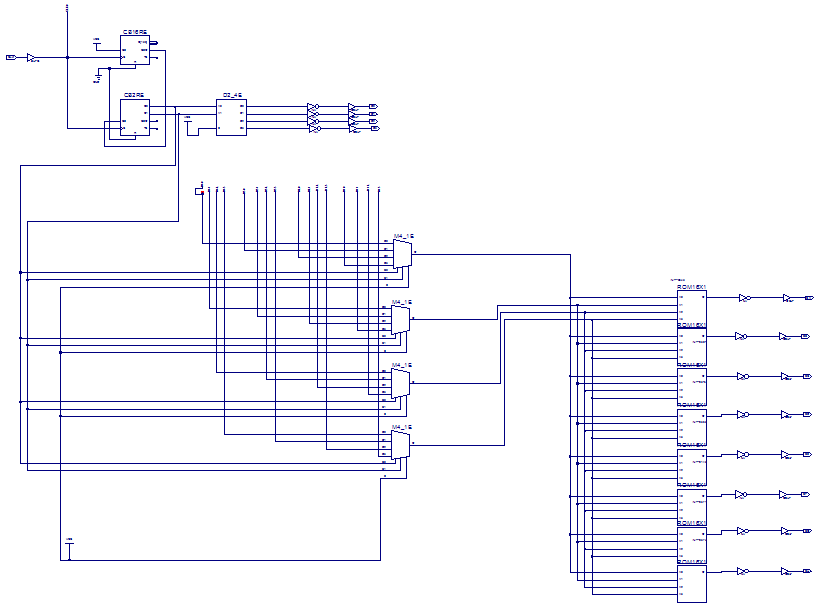
\includegraphics[width=0.45\textwidth]{freq-1}}%
\hspace{8pt}%
%
\subfloat[][]{%
\label{fig:freq-2}%
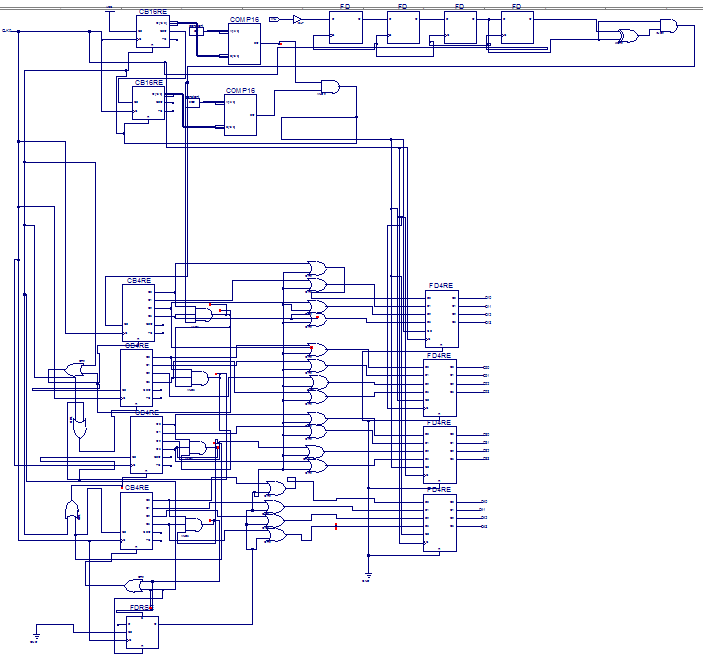
\includegraphics[width=0.45\textwidth]{freq-2}}%
\hspace{8pt}%
%
\caption[Схема частотомера.]{Схема частотомера:
\subref{fig:freq-1} схема динамической индикации; %
\subref{fig:freq-2} схема измерителя частоты} %
\label{fig:freq}%
\end{figure}

Был разработан проект для реализации измерения частоты внешнего периодического сигнала. Проект состоит из двух листов схем (\autoref{fig:freq}).

\subsubsection{Схема динамической индикации}

Первый лист содержит схему динамической индикации, которая состоит из:

\begin{enumerate}[label=\asbuk*)]

\item делителя частоты до значения порядка 1кГц;

\item счетчика индикаторов, значение в котором определяет номер активного в данный момент времени индикатора приставки \enquote{блок динамической индикации};

\item дешифратора, включающего активный индикатор и подключающего его по управлению;

\item четырех 4-мультиплексоров, в зависимости от номера текущего индикатора подключающих соответствующий канал данных (цифра / символ) к преобразователю кодов;

\item преобразователя кодов, выполненного на восьми элементах постоянной памяти \eng{ROM16X1}, образующих таблицу $16 \times 8$, строки которой определяют десять десятичных цифр и шесть дополнительных символов, а восемь столбцов соответствуют восьми сегментам индикатора.

\end{enumerate}

Соответствующие выходы преобразователя кодов подключены к соответствующим сегментам индикатора.

\subsubsection{Схема измерения частоты}

Второй лист содержит схему измерения частоты, которая состоит из следующих частей.

\begin{enumerate}[label=\asbuk*)]

\item Формирователь секундных временных интервалов (см. \autoref{sec:time-interval-generator}).

\item Формирователь коротких импульсов. Производит преобразование длинных импульсов внешнего измеряемого сигнала в короткие счетные импульсы в моменты положительных перепадов измеряемого сигнала. Построен на одном \eng{D}-триггере по принципу сравнения исходного и \enquote{задержанного} триггером сигналов.

\item Двоично-десятичный счетчик на базе четырех 4-разрядных счетчиков. Предназначен для счета импульсов с формирователя коротких импульсов в десятичной системе счисления. Каждый счетчик соответствует десятичной цифре $0..9$. При накоплении в счетчике значения $9$ в момент поступлении следующего счетного импульса счетчик сбрасывается, а следующий за ним счетчик наращивается на единицу.

\item Схема индикации переполнения. Предназначена для информирования пользователя о слишком большом значении частоты измеряемого сигнала. При переполнении последнего двоично-десятичного счетчика передает на вход буферных регистров коды символов, ответственных за индикацию переполнения.

\item Один 1-разрядный и четыре 4-разрядных буферных регистра. Предназначены для буферизации (сохранения) кодов цифр / символов и сигнала переполнения в промежутках между импульсами формирователя секундных временных интервалов, что необходимо для вывода на индикаторы именно конечного значения частоты или сообщения о переполнении счетчика.

\item Схема формирования звукового сигнала. Для формирования звука используется делитель тактовой частоты до звуковой частоты. При наличии сигнала переполнения в соответствующем буферном регистре выдается разрешение на подачу звукового сигнала на динамик.

\end{enumerate}

\section{Выводы}

При подготовке к работе и в ходе работы были получены теоретические и практические сведения о возможностях ПЛИС и среды разработки цифровых устройств для ПЛИС.

Было синтезировано несколько схем управляющих устройств для ПЛИС \eng{Xilinx} в среде разработки \eng{Xilinx ISE}.

Для реализации проектов потребовались знания из курса \enquote{Электротехника и электроника}, некоторые схемы лабораторного макета и приставки \enquote{блок динамической индикации}.

\begin{thebibliography}{9}

\bibitem{morozov}
  Морозов О.А.
  Основы цифровой электроники и программируемая логика: Учебное пособие. ---
  Нижний Новгород: Нижегородский госуниверситет,
  2014. ---
  127 с.

\bibitem{sorochtin}
  Сорохтин Е.М.
  Реализация цифровых управляющих систем на основе программируемых логических интегральных схем: Методическое пособие. ---
  Нижний Новгород: Издательство Нижегородского госуниверситета,
  2007. ---
  44 с.
\end{thebibliography}